\documentclass[10pt,a4paper]{article}
\usepackage[utf8]{inputenc}
\usepackage{graphicx}
\usepackage[top=1in, bottom=1.25in, left=0.75in, right=0.75in]{geometry}

\title{ELEC2103 - Electronics Project preliminary meeting}
\author{Bronchain Olivier \\ Schellekens Vincent \\ Group 7}
\date{\today}

\begin{document}
\maketitle

\section{Report}
\subsection{Game description}
The game is a two-player turn-based strategy game. The concept of the game is inspired by the legendary PC strategy games of the Age of Empires series; of course the concept will be greatly simplified. The two players are RED and BLUE, and will play by turns. The player that is currently playing his turn (denoted by A for the rest of this report) will have the MTL device, while the other player will be handed the LT24 screen. Between turns, the players will have to exchange the screens : a message will be displayed on the screens to indicate this to the players; a multi-touch gesture will have to be performed by player A to indicate that he has the MTL device in his hands and is ready to play. Meanwhile, the website will be used to display several information about the game to the players : the amount of gold of each player, the amount of soldiers, the number of buildings left...

\paragraph{Goal of the game and map layout}
The figure \ref{coucou} presents the map of the game : it consists of two zones : the map (in red) and the menu bar (in green). Each player has three buildings : (the Barracks (B), the Town (T) and the University (U)) and some warriors (indicated by circles). The goal of the game is to move the warriors across the map to destroy the enemy buildings : once all three enemy buildings are destroyed, the player has won. 

\begin{figure}[h!]
    \centering
    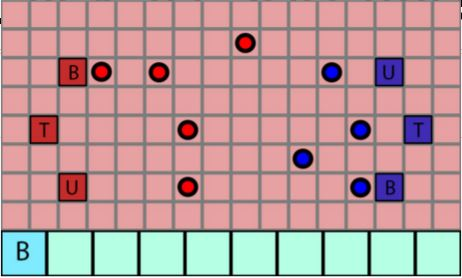
\includegraphics[width = 0.5 \textwidth]{lol}
    \caption{Map layout (on the MTL device)}
    \label{coucou}
\end{figure}

\paragraph{Buildings and their effects}
The buildings each have different purposes. Of course, a destroyed building cannot be used anymore. To use a building, the player has to select the building and then select the action in the menu bar (that will change according to the element of the map the player has selected).

\begin{itemize}
\item Barracks : produces warriors in exchange of \textbf{gold}
\item Town : produces \textbf{gold} and can be improved
\item University : \textbf{gold} can be used here to improve the warriors : for example, make them faster or harder to beat in combat.
\end{itemize}

\paragraph{Moving and fighting with warriors}
Warriors can move across the map : to do that the player will select the warrior and then tilt the screen : using the accelerometer of the FPGA associated with the MTL device, the warrior will then move in the according direction. Fighting between warriors triggers a minigame in which both players will have to find a hidden tile in a 3x4 tile grid by revealing their content by touching each tile. The LT24 screen will thus be used for combat between warriors, but between combats it will display hints for player B.



\subsection{Block Scheme}
    In order to implement our game we will use the block scheme in Figure  \ref{Block}. \\
    \begin{figure}[h!]
        \centering
        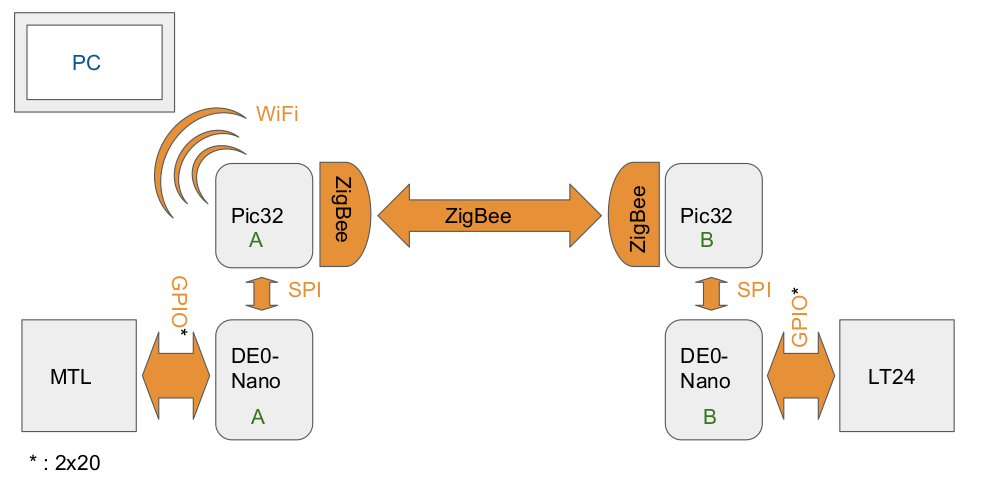
\includegraphics[width = 0.8 \textwidth]{lol3.png}
        \caption{Complete block scheme \label{Block}}
    \end{figure}
    During the game, the following steps are followed:
    \begin{itemize}
        \item \texttt{Before the round:}
                \begin{itemize}
                        \item A and B are independent. The DE0-Nano A communicate via SPI with the PIC32 A (resp. B).
                        \item A and B also communicate with their own screen (MLT for A and LT24 for B).
                        \item A and B display a message mentioning that they are waiting the new round.
                        \item When A received a message from user asking for a new round, A send this information to PC via WiFi and B via ZigBee to start the new round.
                \end{itemize}
        \item \texttt{During the round:}
                \begin{itemize}
                        \item A and B are independent.
                        \item A send message via WiFi to PC to update his behaviour.
                        \item When a new fight occurs, A send a message to B with information like pv etc.
                \end{itemize}
        \item \texttt{During a fight:}
                \begin{itemize}
                        \item A send a message to be for the beginning of the round.
                        \item A and B start a timer (timerA and timerB). A start it when he send the message  and B when he receive it.
                        \item When A and B finish the fight,  they each stop the timer and send it to the other user. The winner it the user with the smallest timer.
                        \item At the end of the fight, A send a message via WiFi to PC to update his behaviour
                \end{itemize}
        \item \texttt{At the end of the round:}
                        \begin{itemize}
                        \item A send a message to B and PC to advertise the end of the round.
                        \end{itemize}
    \end{itemize}

\newpage
\section{Project specifications}

\begin{figure}[h!]
\centering
\begin{tabular}{|p{0.1\textwidth}||p{0.3\textwidth}|p{0.5\textwidth}|}
    \hline
    Week & Course subject & Goal to acheive   \\
    \hline \hline 
    1   &  Tutorial and first use of the touch screens &  Implementation of a sprite and drive an image at the touched point. Being able to retreive the information of the accelerometer of the FPGA. \\ \hline 
    2   &  First use of the Zigbee + WiFi wireless communications & Choose an information on A to display on B and PC. Design of the website and implement communication with it.  \\ \hline 
    3   &  Simple demo of the complete electronic system & Improve the previous topics. Time synchronization between FPGA A and B. \\ \hline 
    4   &  Design of the game &  Review the game according to the possibilities of the system implemented in Week 3. begin working on the map and mini-game.  \\ \hline 
    5   &  Design of the hardware accelerator &  Show all the map on the screen and menu. Display hints on LT24.  \\ \hline 
    6   &  Implementation of the hardware accelerator 1/2 &  Being able to move element on the map with a reasonable delay (Not rewrite all the time the map). Being able to use the accelerator to control the movement on the map. \\ \hline 
    7   &  Implementation of the hardware accelerator 2/2 &  Implementation of the mini-game that occurs during the fight \\ \hline 
    8   &  Introduction of the Real-Time OS &  Implementation of all the rules of the game using the Real-Time OS.  \\ \hline 
    9   &  Test of the game with all specifications 1/2 &   A first clean version of the game. Some delay or bugs are allowed. \\ \hline 
    /   &  Optimization &  Optimization - Test of the game to report bugs -\\ \hline 
    /   &  Optimization &  Optimization - Test of the game to report bugs - \\ \hline 
    10  &  Optimization &  Optimization - Test of the game to report bugs -\\ \hline 
    11  &  Presentation, Demonstration and Drink  &  Report writting  \\ \hline 
\end{tabular}
\caption{Planning of the project}
\end{figure}
\end{document}
